\chapter{绪论}

\section{研究背景及意义}

\subsubsection{选题背景}

预训练模型是已经用广泛的样本训练过的模型。它已经在一个大型数据集上针对特定任务进行了训练。
% 
这个数据集可以是多种形式的,例如图像、文本或音频等。预训练模型的训练过程会产生一种通用的特征表示,这些特征可以被用来执行类似任务的新数据。
% 
从头开始训练一个深度学习模型可能需要花费数周或数月的时间,特别是在缺乏大量数据集的情况下(如BERT~\ucite{devlin2018bert}, GPT-3~\ucite{brown2020language})。
% 
在像ImageNet这样的大型数据集上训练神经网络,该数据集包含1000个类别的1400多万张图片,在这样的数据集上重新训练这样的模型是一种很大的开销。
% 
使用预训练模型可以作为模型的起点,这意味着,当为一个新任务微调预训练的模型时,我们不必从随机权重开始。
% 
而是可以使用预训练的权重作为初始化,然后只训练后面的特定于新任务的层。这需要更少的数据和训练时间。
% 
这可以节省大量的时间和精力。此外预训练模型有其他方面的优势。
% 
它们可以将知识从一般领域转移到特定领域。神经网络的浅层倾向于学习一般的特征,如边缘和形状,而后深则学习更具体的特征。
% 
因此,在一般图像上训练的预训练模型可以提供一般的低层次特征,然后你只需要为你的具体任务重新训练后面的层。这就是所谓的迁移学习。
% 
近年来,学术界和工业界都对开发精度更高,参数量更大的预训练模型感兴趣,因为采用较大的模型会带来更高的准确性。
% 
如图\ref{fig-dl}所示,近年机器学习模型参数量近几年呈现爆炸式增长。远远超出了常用GPU的显存限制(通常只有40-80GB,如Nvidia A100\ucite{nvidia_a100}),这也对我们如何快速,高效的训练模型提出了全新的挑战。

\begin{figure}[t]
\centering
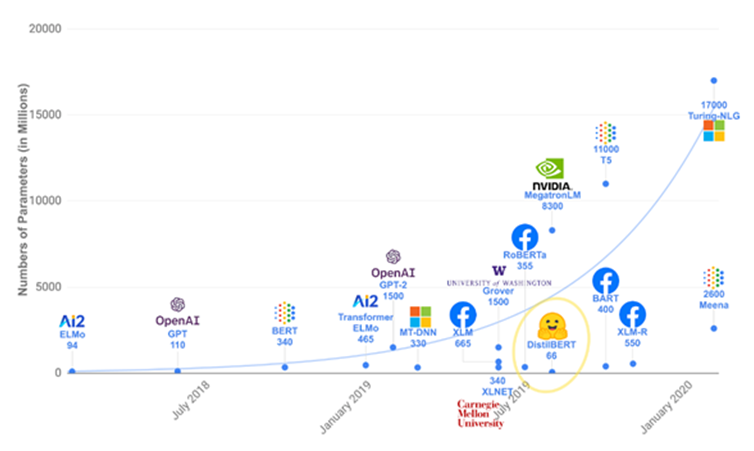
\includegraphics[width=0.7\linewidth]{fig1.png}
\caption{深度学习模型参数显著增长}
\label{fig-dl}
\end{figure}


研究人员表明,较大的模型会带来更高的准确性。
% 
从过去几年深度神经网络 (DNN) 驱动的机器学习技术的快速发展来看,研究者们发现加入更多 DNN 模型参数是最直接但不太复杂的方法之一提高 ML 算法的性能\ucite{kaplan2020scaling}。
% 
然而,DNN 模型容量通常受到计算资源和能源成本的限制\ucite{sharir2020cost}。
% 
根本原因是 DNN 的密集架构,其中计算成本通常与参数数量成线性比例。
% 
为了解决这种问题,混合专家 (MoE)~\ucite{lepikhin2020gshard} 在 DNN 中被广泛使用,它通过使用多个并行子模型(混合专家)引入了稀疏架构,其中每个输入经过门网络,动态选择并转发给少数专家处理。
% 
专家混合似乎有望将模型扩展到极端尺寸。
% 
如图\ref{fig-moe-training} 所示,与直接将小模型缩放为大密集模型不同,MoE\ucite{lepikhin2020gshard} 模型由许多小模型组成,即专家。
% 
训练样本被送入不同的专家,由轻量级可训练门网络动态选择。
% 
在 MoE 中,由于稀疏激活专家,节省了大量额外的计算量,与传统的密集型DNN相比,可以显着增加同一时间段内训练的样本数,提高模型精度。MoE技术是如今将DNN扩展到万亿参数的流行方法之一。

%
MoE混合专家系统是一种稀疏模型,因此其训练过程不同于传统的密集型DNN模型。主要有以下三点挑战:

\begin{itemize}
    \item 
    \textbf{动态激活特性:}
    MoE模型的稀疏激活特性使得它在GPU集群分布式训练时与现有的静态并行策略不匹配。
    因为MoE模型的每个样本只会被激活一个专家(也就是一个子模型),而其他的专家则不会被激活。
    这导致静态并行策略无法充分利用计算资源,因为只有部分计算节点被激活,而其他节点则处于空闲状态。
    % 因此,需要采用动态并行策略来适应MoE模型的稀疏激活特性,以最大限度地利用计算资源。

    \item 
    \textbf{额外通信开销:}
    MoE模型引入了GPU集群节点间额外的All-to-All通信,这种通信方式需要在所有计算节点之间进行数据传输和同步,由于All-to-All通信是一种同步通信方式,因此它会严重影响训练速度和效率。
    但是这种通信方式在MoE模型中是必需的,因为它需要将每个计算节点计算得到的结果进行汇总和组合,以得到最终的预测结果。

    \item 
    \textbf{节点负载不均衡:}
    由于MoE模型中的Gating在训练过程中不断变化,因此数据可能被分配到不同的专家上,导致负载分配不平衡的问题。
    如果某些专家的负载过高,而其他专家的负载过低,就会导致训练时间的延长和模型性能的下降。
    因此,需要根据每个专家的激活情况和计算负载进行动态的数据分配和负载均衡,以确保每个专家的计算负载均衡,并最大限度地利用计算资源。


\end{itemize}

现有的分布式训练框架\ucite{pytorch,deepspeed}对于其稀疏性的结构没有很好的支持,因此本次毕业设置拟设计一种更加高效的MoE训练框架,加速其分布式训练的过程,从而降低训练大规模的MoE模型架构的成本。

\begin{figure}[t!]
\vskip 2ex
\centering
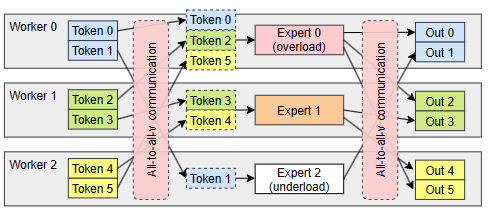
\includegraphics[width=0.69\linewidth]{fig6.png}
\caption{分布式MoE模型训练过程}
\label{fig-moe-training}
\end{figure}


\subsubsection{选题依据}
% 
随着人工智能技术的不断发展,MoE模型在各个领域都具有广泛的应用前景。它可以将多个不同的模型集成起来,以提高模型的性能和泛化能力。
% 
目前MoE模型在语音识别、自然语言处理、计算机视觉等领域都取得了很好的效果。
% 
因此,研究MoE模型的分布式训练和优化策略对于进一步提高模型的训练效率和性能具有重要意义。通过并行化和分布式计算等技术手段,可以加快MoE模型的训练过程,同时提高模型在大规模数据集上的效果。这将有助于应对深度学习任务和数据集日益复杂和庞大的挑战。
% 
此外,研究MoE模型的训练和优化策略不仅对于深度学习领域的研究具有重要意义,还能为各个领域的应用提供更高效和精确的解决方案。通过将多个专家的知识和能力结合起来,MoE模型能够更好地应对现实世界中的复杂问题,并提供更加准确和可靠的预测结果。
% 
因此,对MoE模型的分布式训练和优化策略进行深入研究,还能够在各个应用领域中取得更大的突破,为人工智能技术的进步做出重要贡献。



\section{国内外研究现状}

\subsection{MoE训练系统}
随着MoE训练范式的普及,许多科研机构和企业都开源了MoE训练框架和系统。 
% 
DeepSpeed-MoE 利用多种分布式并行方法结合 MoE 并行性,包括数据并行、张量切片\ucite{shoeybi2019megatron}、Zero内存优化\ucite{rajbhandari2020zero}来训练更大的模型。至于 MoE 的推理,DeepSpeed\ucite{rajbhandari2022deepspeed}设计了一种名为 PR-MoE 的新型稀疏激活模型和模型压缩技术来减小 MoE 模型的大小,以及一种有效的通信方法来优化延迟。 
% 
FastMoE\ucite{he2021fastmoe} 是一个分布式 MoE 训练系统,它提供了一个分层接口和简单的机构,说明如何基于数据并行性和张量切片并行性使用 Megatron-LM\ucite{shoeybi2019megatron} 和 Transformer-XL\ucite{dai2019transformer}。
% 
与 DeepSpeed 的实施不同,FastMoE 使用复杂的优化方法来减少网络流量。
% 
Fairseq-MoE\ucite{ott2019fairseq}  是一个序列建模框架,用于训练用于摘要、翻译和语言建模的自定义模型。
% 
而 Tutel\ucite{hwang2022tutel} 在通信和计算方面进一步优化了 Fairseq 系统,其性能提升了约 40\%。
Tutel 中的优化已集成到 DeepSpeed 中,以促进 MoE 模型训练。

\subsection{MoE数据分派策略}
MoE的核心问题之一是如何设计gating策略,即如何根据输入分配不同的专家网络。不同的gating策略会影响模型的性能、稀疏性、均衡性和公平性。
\begin{itemize}
    \item \textbf{Softmax gating}\ucite{he2021fastmoe}:这是最简单的一种gating策略,它使用一个softmax层来为每个输入分配一个概率分布,表示每个专家网络的权重。这种方法可以看作是多个专家网络合作来产生输出,但是也会导致所有的专家网络都被激活,从而增加计算量和内存消耗。
    \item \textbf{Top-k gating}\ucite{hwang2022tutel}:这种gating策略只选择概率最高的k个专家网络来处理输入,其他的专家网络则被忽略。这种方法可以实现稀疏性,即只有少数的专家网络被激活,从而节省计算量和内存消耗。但是这种方法也会带来一些问题,比如如何确定k的值,以及如何保证每个专家网络都能被充分利用。
    \item \textbf{Noisy softmax gating}\ucite{xu2022survey}:这种gating策略在softmax gating的基础上增加了一个可学习的噪声权重,用来提高不同专家网络的gating均衡性。这种方法可以防止某些专家网络被过度使用或者被忽略,从而提高模型的公平性和泛化能力。
    \item \textbf{Hierarchical softmax gating}\ucite{xu2022survey}:这种gating策略将多个专家网络组织成一个层次结构,每一层都有一个softmax gating来决定下一层的激活。这种方法可以减少softmax gating的计算复杂度,从而提高模型的效率。
    \item \textbf{Hash layer}\ucite{roller2021hash}:这种gating策略使用哈希函数来为每个输入分配一个或多个专家网络,而不需要学习任何参数或者使用额外的损失函数。这种方法可以实现极高的稀疏性和效率,同时保持或者提升模型的性能。
    \item \textbf{Topology-aware gating}\ucite{chen2022ta}: TA-MoE中提出了一种拓扑感知的路由策略,它能够根据网络拓扑的变化动态地调整MoE的数据分派的调度策略。通过基于通信建模的方法,TA-MoE将调度问题抽象为一个优化目标,并得到了适用于不同拓扑结构的近似调度模式。他们设计了一种拓扑感知辅助损失函数,它可以自适应地根据底层拓扑调整数据分派策略,而不会牺牲模型的准确性。
\end{itemize}

\subsection{分布式深度学习训练系统概述}

分布式深度学习训练是一种将一个任务划分为较小的子任务并在多个处理器或设备上同时运行的技术\ucite{ben2019demystifying}。
% 
这种方法可以加快任务的执行速度,特别是当子任务可以在不同的处理器或设备上并行执行时。
% 
在分布式深度学习训练中,我们通过将训练数据和模型参数分布在多个处理器或设备上,然后在多个GPU上同时执行子任务来提高训练速度。
% 
这使我们能够突破单个GPU的内存限制,训练出比单个处理器或设备上所能训练的更大的深度学习模型。
% 
通过将训练过程在多个GPU上并行化,我们有效地增加了可用于训练模型的计算能力。每个GPU在训练数据的一个子集和模型参数的一部分上工作。然后通过汇总各个GPU的结果来建立整体模型。
% 
随着深度学习模型的规模和复杂性不断增加,分布式训练的好处变得更加明显。
% 
更大的神经网络需要更多的数据和计算来优化大量的权重和参数。
% 
通过利用多个GPU,我们可以扩大可用资源的规模,以满足这些大规模模型的需求。

目前,分布式深度学习训练中使用的并行性主要有三种类型:

\begin{itemize}
\item 
\textbf{数据并行性 (Data parallel)\ucite{ben2019demystifying}:}
在数据并行要求整个模型能够装入每个处理器或设备的内存中,这种方案将大规模的数据集分成多个小批次,分别在不同的处理器或设备上并行计算,以提高深度学习模型的训练速度和效率。
% 
在每个训练迭代或历时结束时,模型参数在所有处理器或设备上同步。
% 
更具体地说,每个处理器或设备在其训练数据部分的一批训练样本上工作。
% 
它在这个本地批次上执行前向和后向传播,以计算梯度并更新其模型副本中的权重和偏差。
% 
计算完成之后需要执行同步步骤,来自每个处理器或设备的模型参数被平均到一起(太频繁的同步会因为通信开销而降低训练速度,而太不频繁的同步则会导致独立的模型副本之间出现分歧)。
% 
通过数据并行和模型参数的定期同步,训练数据和计算可以有效地分布在多个处理器或设备上,以加快深度学习模型的训练。
% 
总的来说,数据并行难度相对较低,只需要并行化已有代码,但是其额外的通信开销随着GPU数量增加而增加,大规模训练性能较差。

\begin{figure}[t!]
    \vskip 2ex
    \centering
    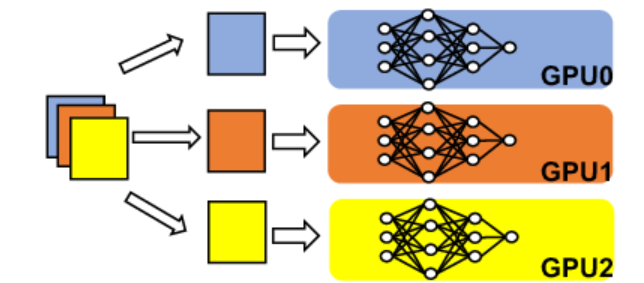
\includegraphics[width=0.7\linewidth]{figures/dataparallel.png}
    \caption{分布式训练-数据并行}
    \label{fig-data-parallel}
    \end{figure}

\item
\textbf{模型并行性 (Model parallel)\ucite{shazeer2018mesh}:}
模型并行可用于训练太大而无法放入单个处理器或设备的内存中的模型,但是需要处理器或设备之间进行更多通信模型的参数分割到多个GPU卡或服务器上训练。
% 
这种方法将复杂的深度学习模型分割成独立的子模型,并分配到多张GPU卡或服务器上,从而减少单个设备的计算负担。
% 
在每张GPU计算完成对应部分之后,需要将中间的激活值通过网络传输(NCCL\ucite{nccl})的方式发送给其他GPU参与后续阶段参与计算。
% 
使用模型并行需要对模型进行重构以分割参数,因此相应的并行度比较高。
% 
这种方式可以利用更多的计算资源来加速非常大模型的训练,但是参数分割和同步亦需要投入额外工作并存在较高的通信开销。
% 
总的来说,模型并行适合那些模块化清晰且参数易于分割的深度学习模型,并且可以更好地随处理器数量线性缩放。

\begin{figure}[h!]
    \vskip 2ex
    \centering
    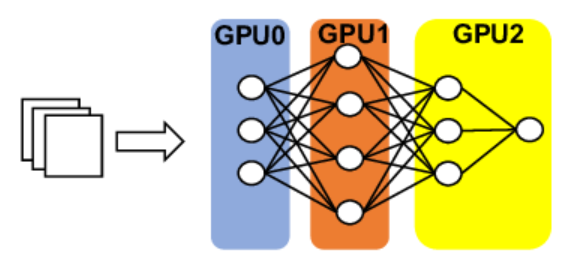
\includegraphics[width=0.7\linewidth]{figures/modelparallel.png}
    \caption{分布式训练-模型并行}
    \label{fig-model-parallel}
    \end{figure}

\item
\textbf{流水线并行 (Pipeline parallel)\ucite{huang2019gpipe}:}
流水线并行是一种通过将深度学习模型划分为多个独立阶段,并行执行不同阶段来加速训练模型的技术。具体操作包括:
% 
首先将模型分割成多个连续的阶段,如Embedding层、卷积层、池化层等
% 
并将一个Batch的数据划分为多个Macro-Batch分配给不同的阶段进行计算。
% 
当一个Macro-Batch通过一个阶段后,将结果传递给下个阶段,直至所有的Macro-batch通过流水线。
% 
不同阶段的计算可以同时执行,形成 computaional pipeline。
% 
整个Batch全部通过后,损失函数和梯度计算在最后一个阶段完成。
% 
流水线并行适用于很大的模型,超出单个GPU容量。它可以利用多个GPU来加速训练。
% 
流水线并行的优点是可以扩展到多个GPU来利用更多计算资源,利用计算资源更有效率。
% 
但是它主要挑战是需要更严格的同步不同阶段的计算,部分阶段可能存在空转,需要通过调整Macro-Batch大小来缓解。
% 
通常模型并行与流水线并行可能一起使用,以更好的平衡流水线并行中各个阶段的计算负载与数据通信开销。

\begin{figure}[t!]
    \vskip 2ex
    \centering
    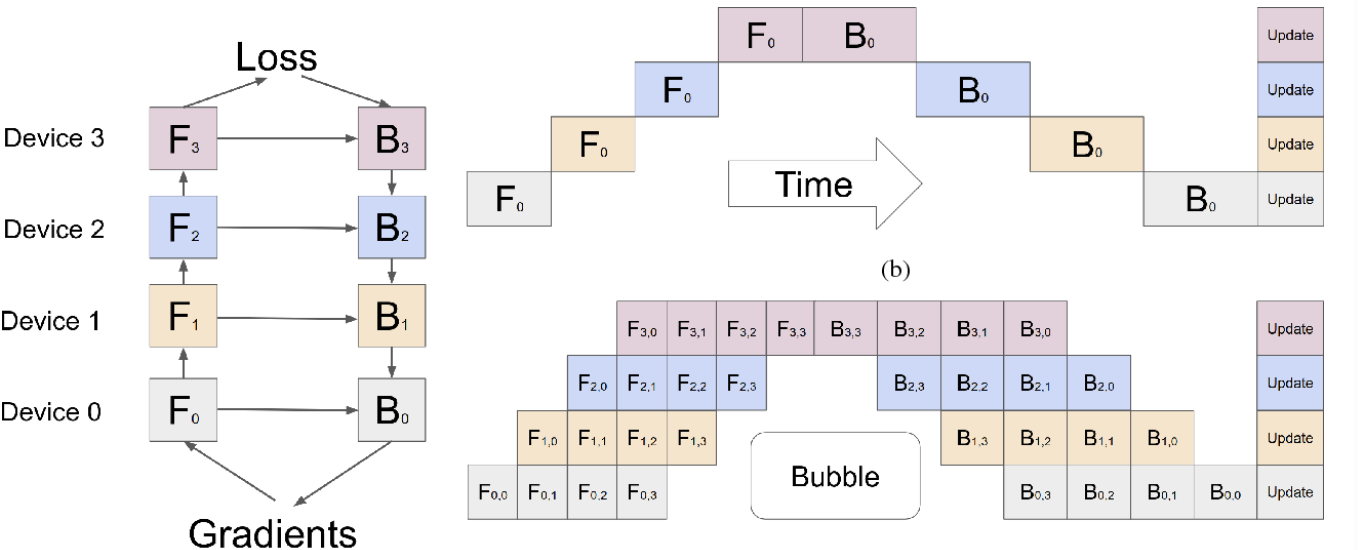
\includegraphics[width=0.7\linewidth]{figures/pipelineparallel.png}
    \caption{分布式训练-流水线并行}
    \label{fig-pipeline-parallel}
    \end{figure}


\end{itemize}

并行训练模型时,我们需要通过合理的任务划分和调度来优化深度学习训练的效率和可扩展性,并根据深度学习模型本身的特点和可用的硬件资源选择最佳的并行方案。从而在保证模型精度的同时,实现训练速度提升,支持更大规模的训练,以及提高可靠性和容错性。
% 
这种方式可以更充分地利用计算资源,提高深度学习模型的训练效率和可扩展性,从而适应越来越复杂和庞大的深度学习任务和数据集的需求。

\section{本文组织结构}

本文的组织结构如下:

本文的第二章是MoE训练过程的概述。
% 
该章主要介绍了MoE混合专家模型在分布式深度学习训练中的主要过程,分析了其正向反向传播的计算过程,并解释了为什么MoE模型与现有传统集中式训练系统的不匹配。

本文的第三章是基于动态路由的数据分派策略的设计方式。
%
该章首先分析了现有的数据分派策略的主要方式,并总结了现有设计的不足之处。进而更进一步,给出了我们设计的基于动态路由的数据分派策略具体的方案架构,包括方案的详细流程和性能分析。


本文的第四章为基于网络拓扑的自动负载均衡策略方案设计。
%
该章首先分析了现有GPU数据中心网络拓扑。并结合每个专家在训练过程的负载变化现象,建立模型寻找最佳的负载均衡方案设计。


本文的第五章为系统实现以及实验结果展示。
%
该章给出了整体的设计方案以及实验结果展示。

本文的第六章为总结与展望。
%
该章总结了本文的主要贡献,以及对未来工作的展望。


\section{本章小结}

本章首先对论文选题的背景和研究意义进行讨论,提出了稀疏混合专家MoE模型对于现有深度学习训练系统的挑战,然后分别介绍了本文的研究点。
%
随后对国内外研究现状进行了简要的介绍。

\endinput